% !TeX root = main.tex
\lecture{1}{Wed 01 Oct 2025 11:00}{Intro to Waves and SHM Recap}

\subsection*{Course Objectives}
\begin{itemize}
    \item Have a sound understanding of basic wave properties
    \item Have a basic understanding of interference effects, inc diffraction
    \item Be able to use simple geometric optics and understand the fundamentals of optical instruments.
\end{itemize}


\subsection*{Recommended Textbooks}
\begin{enumerate}
    \item University Physics, Young and Freedman (Ch 15, 16 for Waves, Ch 33-36 for Optics)
    \item Physics for Scientists and Engineers (Ch 20, 21 for Waves, Ch 22-24 for Optics)
    \item 5e, Tipler and Mosca, (Ch 15, 16 for Waves, 31-33 for Optics)
    \item Fundamentals of Optics, Jenkins and White
    \item Optics, Hecht and Zajac
\end{enumerate}

\paragraph{What is a wave?} Waves occur when a system is disturbed from equilibrium and the disturbance can travel from one region to another region. Waves carry energy, but do not move mass. The course aim is to derive basic equations for describing waves, and learn their physical properties.

\subsection*{Periodic Motion}
Waves are very linked to periodic motion. Therefore we recap periodic motion first.

It has these characterstics:
\begin{itemize}
    \item A period, $T$ (the time for one cycle)
    \item A frequency, $f$, the number of cycles per unit time ($f = \frac{1}{T}$)
    \item An amplitude, $A$, the maximum displacement from equilibrium.
\end{itemize}

Periodic motion continues due to the restoring force. When an object is displaced from equilibrium, the restoring force acts back towards the equi point. The object reaches equi with a non-zero speed, so the motion continues past the equi point and continues forever.

\subsection*{Energy}
Periodic motion is an exchange between potential and kinetic energy, with no energy loss. Energy is conserved.

\subsection*{Simple Harmonic Motion}
If the restoring force is directly proportional to the displacement $F = -kx$, then the periodic motion becomes Simple Harmonic Motion and the object is called a harmonic oscillator.

In a single dimension, displacement is given by:
\[
    x = A \cos(\omega t + \phi)
\]
Where $\omega = 2 \pi f$ is the angular velocity, and $\phi$ is the phase angle. In cases like this, where the phase angle is $90 \deg$ we can simplify to $x = -A \sin(\omega t)$
\begin{figure}[H]
    \centering
    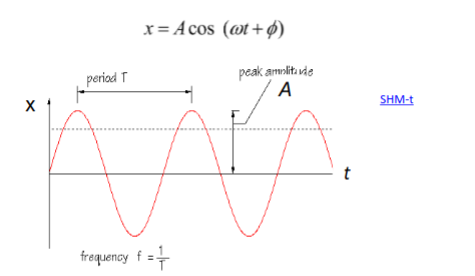
\includegraphics{figures/phaseangle.png}
    \caption{A Phase Angle of 90}
\end{figure}

\subsection*{More SHM Equations}
\textbf{Velocity}

\[
    v_x = \frac{dx}{dt} = - \omega A \sin(\omega t + \phi)
\]

\textbf{Acceleration}

\[
    a_x = \frac{d v_x}{dt} = \frac{d^2 x}{dt^2} = - \omega^2 A \cos(\omega t + \phi)
\]

Both properties are signed to indicate direction, as they are both vectors.



